\documentclass[12pt,a4paper]{report}
\usepackage[italian]{babel}
%\usepackage[T1]{fontenc} % Riga da commentare se si compila con PDFLaTeX
\usepackage{geometry}
\usepackage{graphicx}
\usepackage{hyperref}
\usepackage[utf8]{inputenc}
\usepackage{lipsum} % genera testo fittizio
\usepackage[nottoc,numbib]{tocbibind}
\usepackage{titlesec}
\usepackage{cochineal}
\usepackage[cochineal]{newtxmath}
\usepackage[simplified]{pgf-umlcd}
\usepackage{float}
\usepackage{wrapfig,lipsum}
\usepackage{fancyhdr, etoolbox}
\usepackage{xcolor}
\usepackage{listings}
\usepackage{xparse}
\usepackage{url}
\usepackage{setspace}
\usepackage{longtable}
\usepackage{etaremune}
\usepackage{booktabs}
\usepackage{subfig}
\usepackage[edges]{forest}
\definecolor{folderbg}{RGB}{124,166,198}
\definecolor{folderborder}{RGB}{110,144,169}
\newlength\Size
\setlength\Size{4pt}
\tikzset{%
  folder/.pic={%
    \filldraw [draw=folderborder, top color=folderbg!50, bottom color=folderbg] (-1.05*\Size,0.2\Size+5pt) rectangle ++(.75*\Size,-0.2\Size-5pt);
    \filldraw [draw=folderborder, top color=folderbg!50, bottom color=folderbg] (-1.15*\Size,-\Size) rectangle (1.15*\Size,\Size);
  },
  file/.pic={%
    \filldraw [draw=folderborder, top color=folderbg!5, bottom color=folderbg!10] (-\Size,.4*\Size+5pt) coordinate (a) |- (\Size,-1.2*\Size) coordinate (b) -- ++(0,1.6*\Size) coordinate (c) -- ++(-5pt,5pt) coordinate (d) -- cycle (d) |- (c) ;
  },
}
\forestset{%
  declare autowrapped toks={pic me}{},
  pic dir tree/.style={%
    for tree={%
      folder,
      font=\ttfamily,
      grow'=0,
    },
    before typesetting nodes={%
      for tree={%
        edge label+/.option={pic me},
      },
    },
  },
  pic me set/.code n args=2{%
    \forestset{%
      #1/.style={%
        inner xsep=2\Size,
        pic me={pic {#2}},
      }
    }
  },
  pic me set={directory}{folder},
  pic me set={file}{file},
}
\include{json-lang}
\usepackage[style=numeric-comp,useprefix,hyperref,backend=bibtex]{biblatex}


\NewDocumentCommand{\codeword}{v}{%
    \texttt{\textcolor{blue}{#1}}%
}

\lstset{language=C,keywordstyle={\bfseries \color{blue}}}

%\usetikzlibrary{calc}
\pagestyle{fancy}

\fancyhead{}
\fancyhead[OL]{\ifnumodd{\value{page}}{\slshape \leftmark}{\slshape SEZIONE \rightmark}}
\fancypagestyle{mystyle}{
    \fancyhead[OL]{\slshape \leftmark}
}
\fancyfoot[C]{\thepage}

\fontfamily{bch}\selectfont

% Taken from Lena Herrmann at
% http://lenaherrmann.net/2010/05/20/javascript-syntax-highlighting-in-the-latex-listings-package

\usepackage{color} %use color
\definecolor{mygreen}{rgb}{0,0.6,0}
\definecolor{mygray}{rgb}{0.5,0.5,0.5}
\definecolor{mymauve}{rgb}{0.58,0,0.82}

%Customize a bit the look
\lstset{ %
backgroundcolor=\color{white}, % choose the background color; you must add \usepackage{color} or \usepackage{xcolor}
basicstyle=\footnotesize, % the size of the fonts that are used for the code
breakatwhitespace=false, % sets if automatic breaks should only happen at whitespace
breaklines=true, % sets automatic line breaking
captionpos=b, % sets the caption-position to bottom
commentstyle=\color{mygreen}, % comment style
deletekeywords={...}, % if you want to delete keywords from the given language
escapeinside={<@}{@>}, % if you want to add LaTeX within your code
extendedchars=true, % lets you use non-ASCII characters; for 8-bits encodings only, does not work with UTF-8
frame=single, % adds a frame around the code
keepspaces=true, % keeps spaces in text, useful for keeping indentation of code (possibly needs columns=flexible)
keywordstyle=\color{blue}, % keyword style
% language=Octave, % the language of the code
morekeywords={*,...}, % if you want to add more keywords to the set
numbers=left, % where to put the line-numbers; possible values are (none, left, right)
numbersep=5pt, % how far the line-numbers are from the code
numberstyle=\tiny\color{mygray}, % the style that is used for the line-numbers
rulecolor=\color{black}, % if not set, the frame-color may be changed on line-breaks within not-black text (e.g. comments (green here))
showspaces=false, % show spaces everywhere adding particular underscores; it overrides 'showstringspaces'
showstringspaces=false, % underline spaces within strings only
showtabs=false, % show tabs within strings adding particular underscores
stepnumber=1, % the step between two line-numbers. If it's 1, each line will be numbered
stringstyle=\color{mymauve}, % string literal style
tabsize=1, % sets default tabsize to 2 spaces
title=\lstname, % show the filename of files included with \lstinputlisting; also try caption instead of title
}
%END of listing package%

\definecolor{darkgray}{rgb}{.4,.4,.4}
\definecolor{purple}{rgb}{0.65, 0.12, 0.82}

%define Javascript language
\lstdefinelanguage{JavaScript}{
keywords={typeof, new, true, false, catch, function, return, null, catch, switch, var, if, while, do, else, case, break, for, of, const, async, await},
keywordstyle=\color{blue}\bfseries,
ndkeywords={class, export, boolean, throw, implements, import},
ndkeywordstyle=\color{darkgray}\bfseries,
identifierstyle=\color{black},
sensitive=false,
comment=[l]{//},
morecomment=[s]{/*}{*/},
commentstyle=\color{purple}\ttfamily,
stringstyle=\color{red}\ttfamily,
morestring=[b]',
morestring=[b]"
}

\lstset{
language=JavaScript,
extendedchars=true,
basicstyle=\footnotesize\ttfamily,
showstringspaces=false,
showspaces=false,
numbers=left,
numberstyle=\footnotesize,
numbersep=9pt,
tabsize=1,
breaklines=true,
showtabs=false,
captionpos=b
}

\definecolor{pblue}{rgb}{0.13,0.13,1}
\definecolor{pgreen}{rgb}{0,0.5,0}
\definecolor{pred}{rgb}{0.9,0,0}
\definecolor{pgrey}{rgb}{0.46,0.45,0.48}

\usepackage{listings}
\lstset{language=Java,
  showspaces=false,
  showtabs=false,
  breaklines=true,
  tabsize=1,
  showstringspaces=false,
  breakatwhitespace=true,
  commentstyle=\color{pgreen},
  keywordstyle=\color{pblue},
  stringstyle=\color{pred},
  basicstyle=\ttfamily,
  moredelim=[il][\textcolor{pgrey}]{$$},
  moredelim=[is][\textcolor{pgrey}]{\%\%}{\%\%}
}


\titleformat{\chapter}[display]{\Huge\bfseries}{}{0pt}{\thechapter.\ }

\graphicspath{{figures/}}
%
%\addtolength{\topmargin}{-.875in} % reduce the default top margin
%\addtolength{\topmargin}{-2cm} % reduce the default top margin
%

\tolerance=1
\emergencystretch=\maxdimen
\hyphenpenalty=10000
\hbadness=10000

%%%%%%%%%%%%%%%%%%%%%%%%%%%%%%%%%%
%                                %
%     Begin Docuemnt [start]     %
%                                %
%%%%%%%%%%%%%%%%%%%%%%%%%%%%%%%%%%
\begin{document}

\newgeometry{margin=1in}
\begin{titlepage}
	\centering
	
\includegraphics[width=0.5\textwidth]{logounipg2021}\par\vspace{1cm}
	\large{Presentazione Progetto di}\par
	\large{\textbf{Virtual Networks and Cloud Computing}}\par
	\small{Corso di Laurea in Ingegneria Informatica e Robotica -- A.A. 2022-2023}\par
	\textsc{\small{Dipartimento di Ingegneria}}\par

	%\vfill
	\vspace{0.5cm}
	docente\par
	Prof.~Gianluca \textsc{Reali}

	\vspace{1cm}
	\vspace{1cm}
	\textbf{\huge{Body Performance Predictor}}\par
	\vspace{0.2cm}
	applicazione a microservizi \textsc{Docker / Kubernetes}\par
	\vspace{7cm}

	\large{studenti}\par
	\vspace{0.2cm}
	\begin{tabular}{ l l l l }
	\large{350400} & \large{\textbf{Tommaso}} & \large{\textbf{Martinelli}} & \large{tommaso.martinelli@studenti.unipg.it}\\
	\large{348158} & \large{\textbf{Paolo}} & \large{\textbf{Speziali}} & \large{paolo.speziali@studenti.unipg.it}\\
	\end{tabular}

	\vfill
	% Bottom of the page
	%{\large \today\par}
	\raggedright
	\small{Data ultimo aggiornamento: \today}
\end{titlepage}
% Ends the declared geometry for the titlepage
\restoregeometry
\normalfont
%%%%%%%%%%%%%%%%%%%%%%%%%%%%
%     Title Page [end]     %
%%%%%%%%%%%%%%%%%%%%%%%%%%%%
\newpage \thispagestyle{empty} \ \newpage
%%%%%%%%%%%%%%%%%%%%%%%%%%
%     Indice [start]     %
%%%%%%%%%%%%%%%%%%%%%%%%%%
\onehalfspacing
\tableofcontents

%%%%%%%%%%%%%%%%%%%%%%%%
%     Indice [end]     %
%%%%%%%%%%%%%%%%%%%%%%%%


\chapter{Introduzione}

Per questo progetto è stata sviluppata un'applicazione web
per la classificazione delle performance fisiche degli utenti.
L'utente inserisce i suoi parametri fisici e riceve in output
la qualità della sua performance fisica, indicata da una lettera:
\begin{table}[H]
  \centering
  \begin{tabular}{@{}ll@{}}
  \toprule
  \textbf{Classe} & \textbf{Qualità}   \\ \midrule
  $A$      & Ottima    \\
  $B$      & Buona     \\
  $C$      & Non buona \\
  $D$      & Pessima   \\ \bottomrule
  \end{tabular}
\end{table}

La classificazione avviene tramite un modello di machine learning
addestrato utilizzando il dataset "Body performance"[metti riferimento].

In aggiunta, l'applicazione consente di inserire nuovi dati di training,
che vengono salvati su un database PostgreSQL insieme al dataset originario.

Al fine di garantire la portabilità e semplificare
la realizzazione e la gestione dell'applicativo,
tutte le sue componenti sono state incapsulate in container Docker.
La gestione dei container è stata affidata,
nella sua seconda implementazione,
all'orchestratore Kubernetes.

\chapter{Container}

Di seguito riportiamo la lista dei container
che contengono i microservizi utlizzati
per costruire l'applicativo e i relativi dettagli implementativi e di
interconnessione.
Tutti i container sono stati realizzati
tramite Dockerfile eccetto per il container del database e di
pgAdmin per cui sono state utilizzate immagini prese direttamente da
Docker Hub.

\begin{figure}[H]
  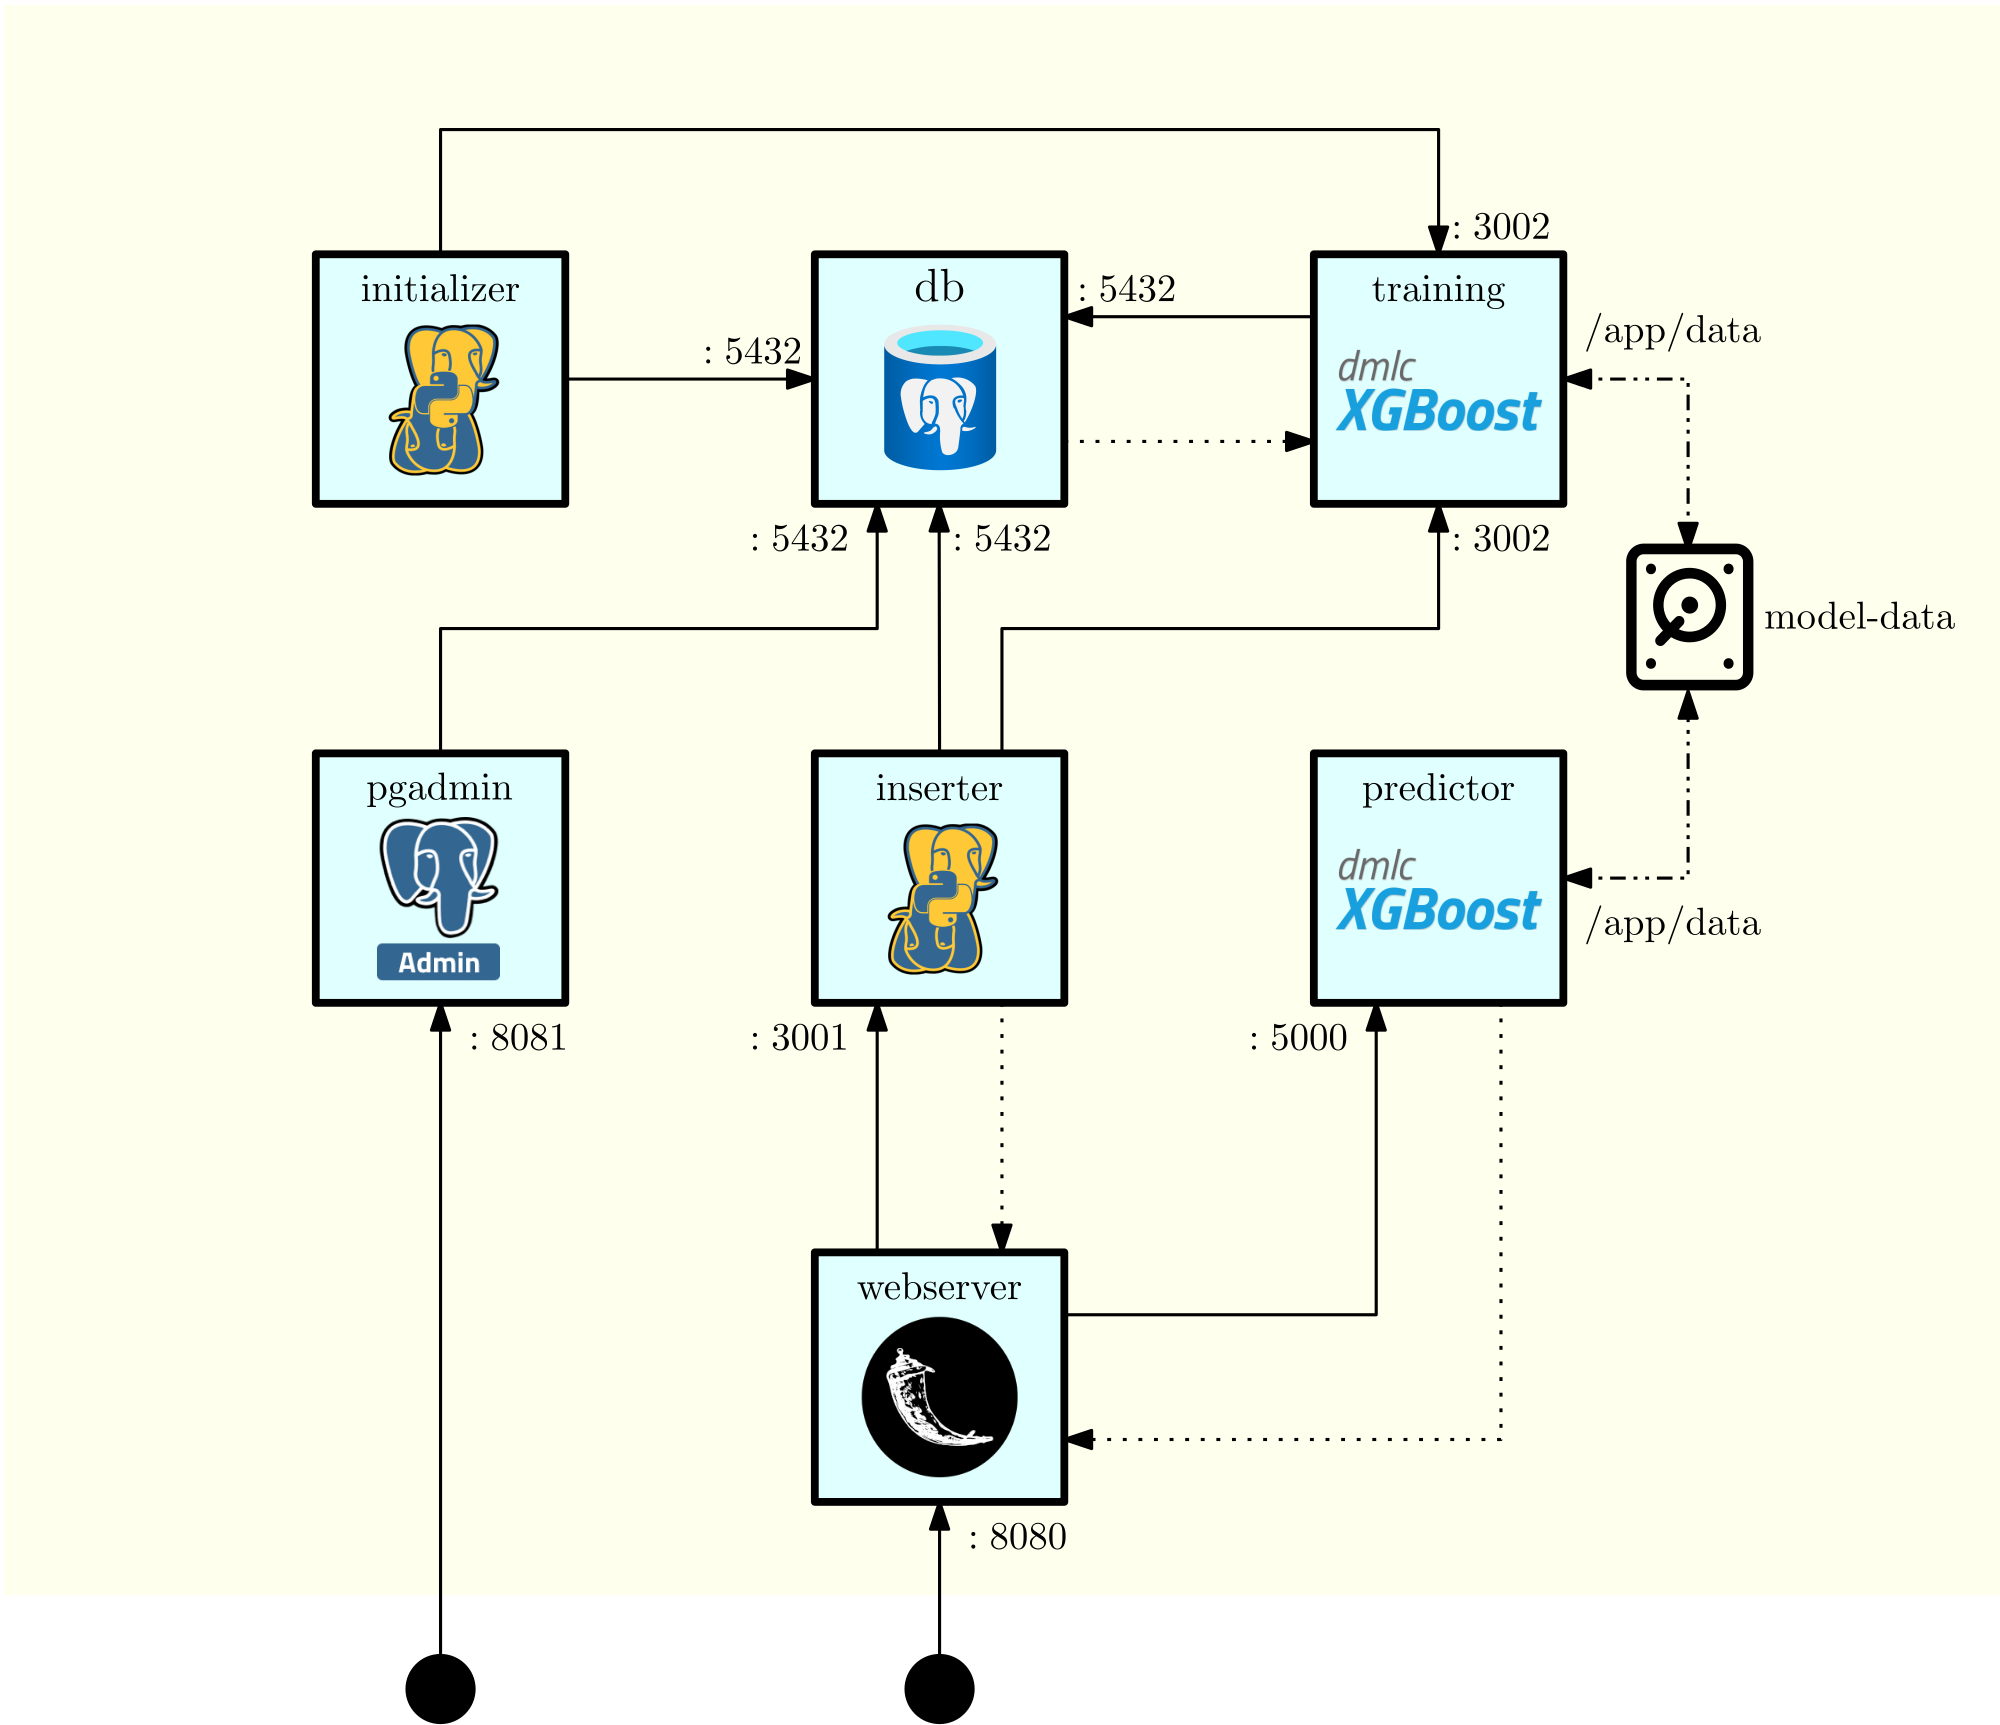
\includegraphics[width=0.8\textwidth]{arch}
  \centering
  \caption{Architettura e collegamenti dell'applicazione}
\end{figure}

\section{Web Server}

Si tratta dell'unico componente che fornisce un'interfaccia grafica
per l'interazione con l'utente.
Per utilizzare l'applicazione web, gli utenti sono tenuti a inserire i seguenti parametri fisici:
\begin{itemize}
\item Età
\item Sesso
\item Altezza
\item Peso
\item Percentuale di grasso corporeo
\item Pressione sanguigna diastolica
\item Pressione sanguigna sistolica
\item Sit and bend forward
\item Gripforce
\item Numero di sit-up
\item Broad jump in centimetri
\end{itemize}

\begin{figure}[H]
  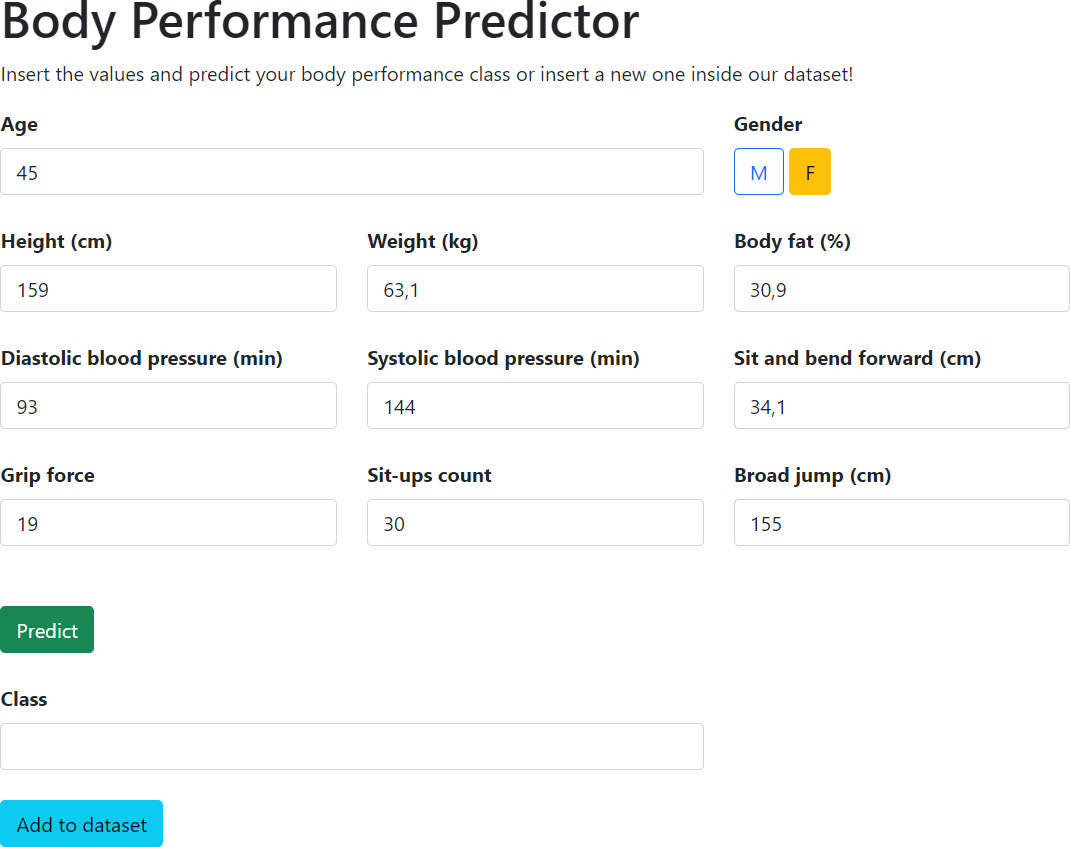
\includegraphics[width=\textwidth]{interfaccia}
  \centering
  \caption{Screenshot dell'interfaccia web dell'applicazione}
\end{figure}

La classe della performance fisica ($A$, $B$, $C$ o $D$) viene predetta
e mostrata in un campo apposito, in alternativa può essere inserita
direttamente dall'utente se è nota e la si desidera caricare
nel database ed includerla negli allenamenti futuri del modello.

Il container è costruito su un'immagine di \textbf{Python} $3.9$
e utilizza il framework \textbf{Flask} per gestire le funzionalità
di un webserver, tra cui fornire tre endpoint con
cui il client può interagire:
\begin{itemize}
  \item \textsc{/}: chiamata GET che restutisce la pagina HTML.
  \item \textsc{/predict}: chiamata POST che restutisce la classe predetta dal modello statistico in risposta ai dati inseriti dall'utente inviati in formato JSON.
  \item \textsc{/insert}: chiamata POST che restutisce l'esito dell'inserimento dei dati (classe inclusa) inseriti dall'utente inviati in formato JSON nel database .
\end{itemize}

\begin{figure}[H]
  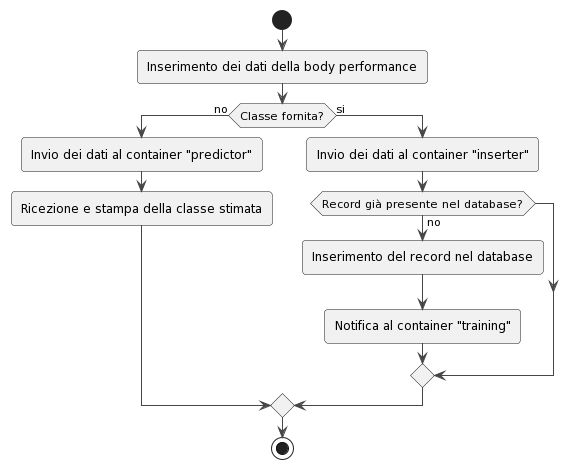
\includegraphics[width=0.8\textwidth]{webserver}
  \centering
  \caption{Flow chart che mostra l'interazione con la pagina web}
\end{figure}


\section{Database}

Si è scelto di utilizzare un container \textbf{PostgreSQL} per diverse ragioni.
Innanzitutto, il dataset utilizzato presenta una struttura fissa
e senza valori $NaN$, si è potuto quindi utilizzare senza problemi
un database relazionale come PostgreSQL senza aggiungere
ulteriore complessità all'applicativo che l'utilizzo di database
NoSQL avrebbero potenzialmente portato.

Inoltre, non si è ritenuto necessario l'utilizzo dello sharding,
poiché il volume dei dati e il carico di lavoro previsto non richiedevano
una distribuzione su più nodi e l'operazione di training avrebbe
comunque richiesto un'operazione di raggruppamento.

Contiene un'unica relazione, denominata \textbf{bodyPerformance},
che contiene la totalità del dataset.
I record con stessi valori (eccetto la classe)
non vengono memorizzati per evitare di influenzare negativamente
le performance del modello.
È possibile monitorare lo stato del database mediante l'uso di
un container \textbf{pgAdmin}, accessibile tramite la porta $8081$.

\section{Training}

Il container è costruito su un'immagine di \textbf{Python} $3.9$
e si occupa, traimte uno script Python, dell'addestramento
del modello di machine learning,
inoltre implementa le funzionalità di un webserver
tramite \textbf{Flask} per permettere
agli altri container di notificarlo
nel caso sia necessario un nuovo training.
Accetta, per questo scopo, richieste GET sulla porta $3002$.

Ad ogni richiesta ricevuta,
interroga il database per farsi restituire
il dataset ed effettua un nuovo addestramento.
Il modello aggiornato è reso disponibile per le predizioni sui dati utente.
Come classificatore è stata scelta la libreria \textbf{XGBoost},
che permette di ottenere, in tempi molto rapidi, risultati soddisfacenti.

\section{Predictor}

Il container è costruito su un'immagine di \textbf{Python} $3.9$
e realizza, tramite \textbf{Flask}, un server
che espone una API REST sulla porta $5000$
e riceve chiamate POST dal web-server contenenti i dati inseriti
dagli utenti.
In seguito alla ricezione dei dati, il predictor esegue una
predizione utilizzando il modello addestrato dal container di training.
Prima di effettuare la predizione, vengono eseguite
opportune trasformazioni sui dati.
Il risultato viene infine inviato al web-server.

\section{Inserter}

Il container è costruito su un'immagine di \textbf{Python} $3.9$
e realizza, tramite \textbf{Flask}, un server
che espone una API REST sulla porta $3001$
e riceve chiamate POST dal web-server contenenti i dati inseriti
dagli utenti.
Si connette al database e inserisce i dati,
l'operazione andrà a buon fine solo
se non esiste un altro record con quei valori
(anche con classe differente).
Al termine, restituisce un messaggio
con l'esito e contatta il container di training per avvisarlo
che è necessario effettuare un nuovo addestramento dopo
l'inserimento dei nuovi dati.

\section{Initializer}

Il container è costruito su un'immagine di \textbf{Python} $3.9$
ed esegue uno script di inizializzazione che ha il compito di creare,
se non presente, la tabella per il dataset nel database e popolarla.
Successivamente, notifica il container di training che può avviare
l'addestramento.
\begin{figure}[H]
  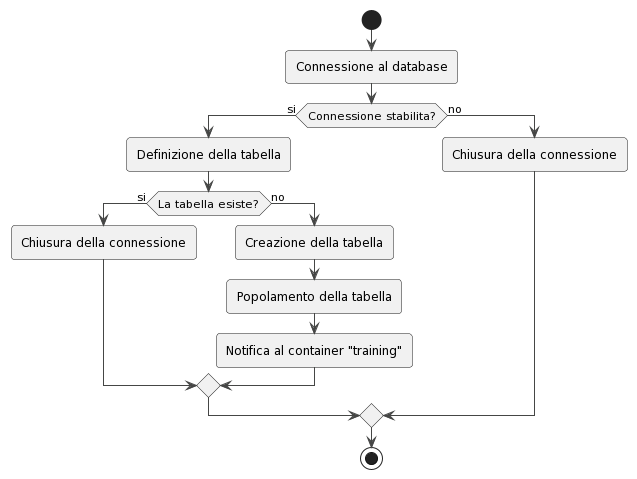
\includegraphics[width=0.8\textwidth]{initializer}
  \centering
  \caption{Flow chart che mostra il funzionamento dello
  script di initializer}
\end{figure}

\chapter{Implementazioni}

Sono state realizzate due diverse versioni dell'applicativo
utilizzando due diverse modalità di orchestrazione,
una con un semplice Docker Compose e l'altra
con l'orchestratore Kubernetes.

\section{Docker Compose}

Docker Compose consente di lanciare contemporaneamente tutti i servizi,
definendo le loro immagini, porte e altri dettagli necessari per il
corretto funzionamento dell'applicazione containerizzata.

In Docker Compose è stato anche possibile definire una rete chiamata
\emph{app\_network}, che consente ai container di comunicare tra loro.
Sono stati utilizzati anche i volumi per garantire la persistenza dei dati.
Ad esempio, per il database è stato necessario utilizzare un volume
per evitare la perdita di eventuali nuovi dati inseriti
dagli utenti e non presenti nel dataset originario
Un altro volume è stato utilizzato per condividere i dati tra
i container training e predictor, in cui vengono salvati il modello
e lo scaler in formato \emph{pickle}. Questo volume garantisce
la disponibilità e la coerenza dei dati, poiché è sempre possibile
richiedere una predizione.
Tuttavia, se tale richiesta viene effettuata durante un addestramento,
verrà utilizzato un modello non ancora aggiornato.
Viene inoltre caricato nel database, come volume, il file CSV
che contiene il dataset originario.
L'intera applicazione è testabile grazie a un file \codeword{init.sh},
che contiene una serie di comandi per creare e avviare i
container tramite il Docker Compose.

\section{Kubernetes}

La versione più recente dell'applicazione è stata orchestrata con
Kubernetes, uno strumento più completo e complesso
rispetto a Docker Compose. Sono stati creati oggetti Deployment,
uno per ogni container Docker, ad eccezione di initializer,
che è stato realizzato con un Job poiché deve essere eseguito
solo una volta e non deve essere riavviato.
Sono stati definiti anche dei Service,
uno per ogni Deployment, per consentire
la connettività tra Pod nella rete interna di Kubernetes
e per esporre le porte $8080$ (webserver)
e $8081$ (pgAdmin) verso l'esterno
tramite il port forwarding di Kubernetes.
In Kubernetes sono stati utilizzati i \emph{PersistentVolumeClaim}
per gestire i volumi,
il volume che contiene il file CSV del dataset è stato incluso tramite
un \emph{config-map}.
Tutti gli oggetti Kubernetes descritti sono stati definiti
utilizzando file YAML.
L'intera applicazione è testabile grazie a un file \codeword{init-k.sh},
che contiene una serie di comandi per creare e configurare gli
oggetti Kubernetes utilizzando i loro file
ed esegue le operazioni di port forwarding.


\hyphenpenalty=0

\cleardoublepage\phantomsection % to fix wrong hyperref to \part{Epilogue}

\end{document}
